\documentclass[mathserif]{beamer}

\usetheme{Berkeley}
\usecolortheme{orchid}
\setbeamertemplate{footline}[frame number]
\setbeamertemplate{navigation symbols}{}

\usepackage[T2A]{fontenc}
\usepackage[utf8x]{inputenc}
\usepackage[english, russian]{babel}
\usepackage{color}
\usepackage{amsmath}
\usepackage{graphicx}
\graphicspath{ {../Images/} }

\title{Поиск семейств оптимальных маршрутов на морских картах}
\author{Иван Громаковский \\
Научный руководитель: А. С. Ковалев}
\institute{Санкт-Петербургский национальный исследовательский университет \\ информационных технологий, механики и оптики}
\date{13 мая 2015}

\begin{document}

\frame{\titlepage}
\note{Здравствуйте!}

\begin{frame}{Цели работы}
    \begin{itemize}[<+->]
        \item Формализация понятия оптимальности
        \item Поиск семейств оптимальных маршрутов для принятия
          решения пользователем
        \item Реализация алгоритма, работающая в режиме реального времени
    \end{itemize}
\end{frame}
\note {
1. И так понятно.
2. Надо что-то придумать тут.
3. Меньше секунды на запрос.

TODO: что-то про то, что достаточно приближённого решения?
}

\begin{frame}{Актуальность задачи}
    Проблемы поиска единственного маршрута:
    \begin{itemize}[<+->]
        \item критерии оптимальности не всегда очевидны и формализуемы
        \item ненадёжность
        \item приводит к повышенной загруженности
    \end{itemize}
\end{frame}
\note {
1. Кратчайший путь не всегда самый лучший. Например, где-то может быть
платный проезд, также нужно учитывать глубину, загруженность. Также у
капитана могут быть личные предпочтения, которые невозможно
формализовать.
2. Если по каким-то причинам проплыть по кратчайшему маршруту не
представляется возможным, возникает проблема, потому что нет альтернатив.
3. Если приложение набирает популярность и все пользуются одинаковыми
(например, кратчайшими) маршрутами, это может приводить повышенной загруженности.

TODO: возможно, что-то ещё можно упомянуть?
}
        
\begin{frame}{Оптимальность маршрутов}
    Назовём семейством оптимальных маршрутов из одной точки в другую 
    максимальное по включению множество путей между этими точками,
    обладающее следующими свойствами:
    \begin{itemize}[<+->]
        \item для любых двух маршрутов найдётся препятствие, размеры
          которого сопоставимы с длиной кратчайшего из маршрутов,
          которое обходится с разных сторон
        \item TODO: получше сформулировать первый пункт
        \item TODO: ещё пункты?
    \end{itemize}
\end{frame}
\note{Слайд не готов}

\begin{frame}{Существующие алгоритмы}
    \only<1-3>{Известные алгоритмы множественного поиска путей в графе
      имеют следующие недостатки:}
    \begin{itemize}
        \item<1-3> разрабатывались для других целей
        \item<2-3> не учитывают реальное физическое расположение
          вершин в графе
        \item<3-3> строят очень похожие маршруты на морских картах
    \end{itemize}
    \only<4-4> {
        \begin{figure}
            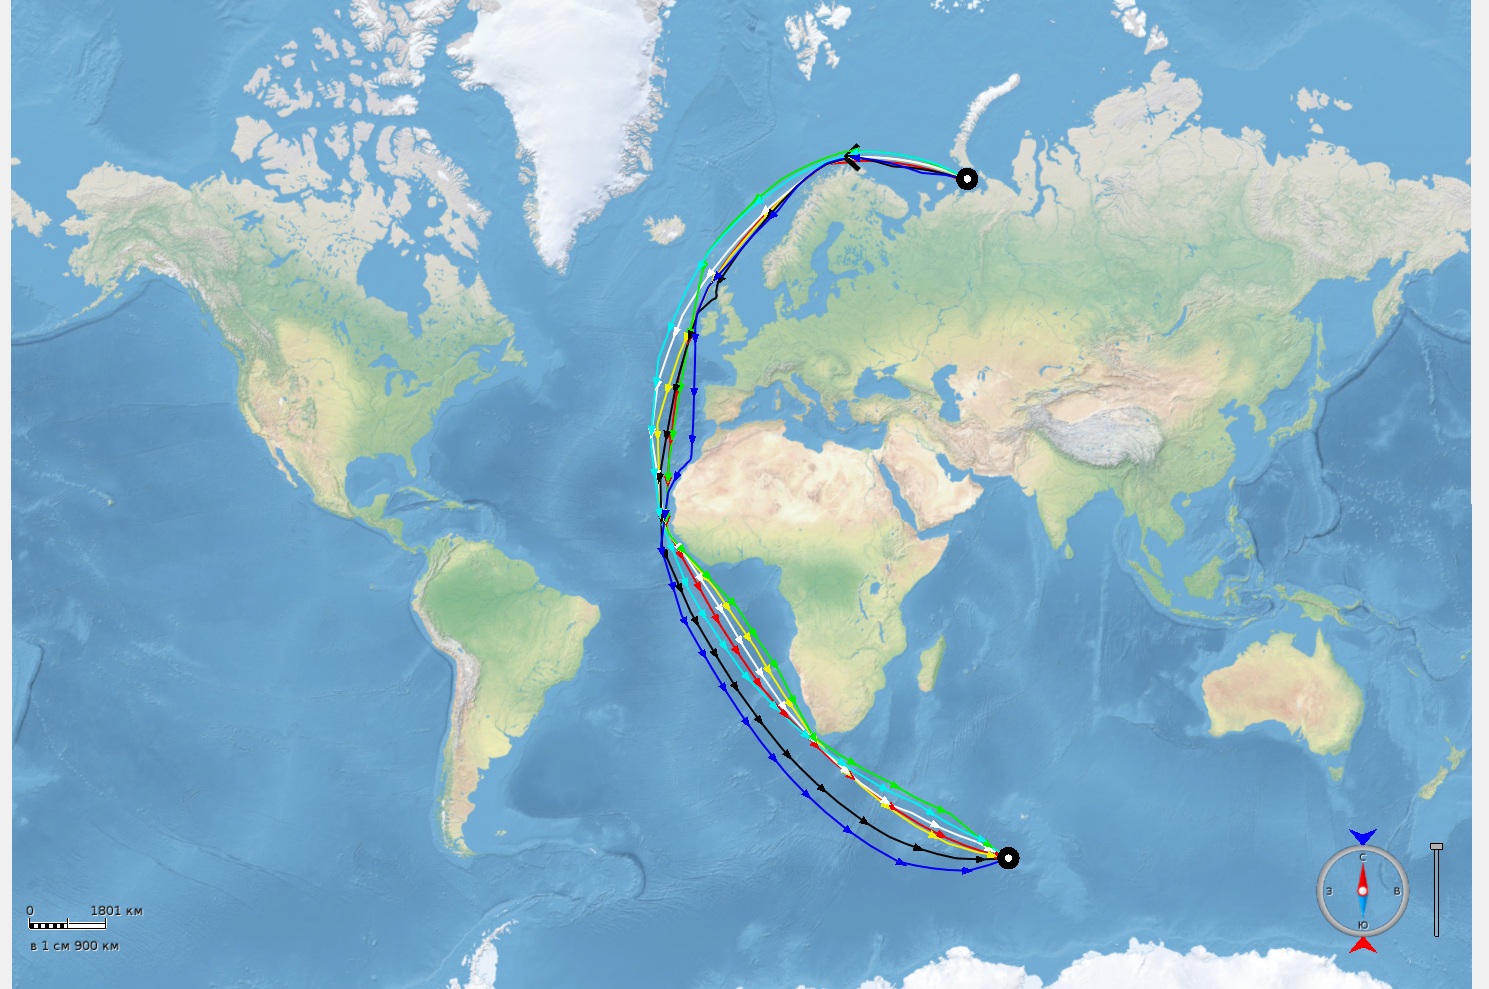
\includegraphics[width=.8\textwidth]{comparison-with-existing-bad}
            \caption{Результат работы существующего алгоритма}
        \end{figure}
    }
    \only<5-5> {
        \begin{figure}
            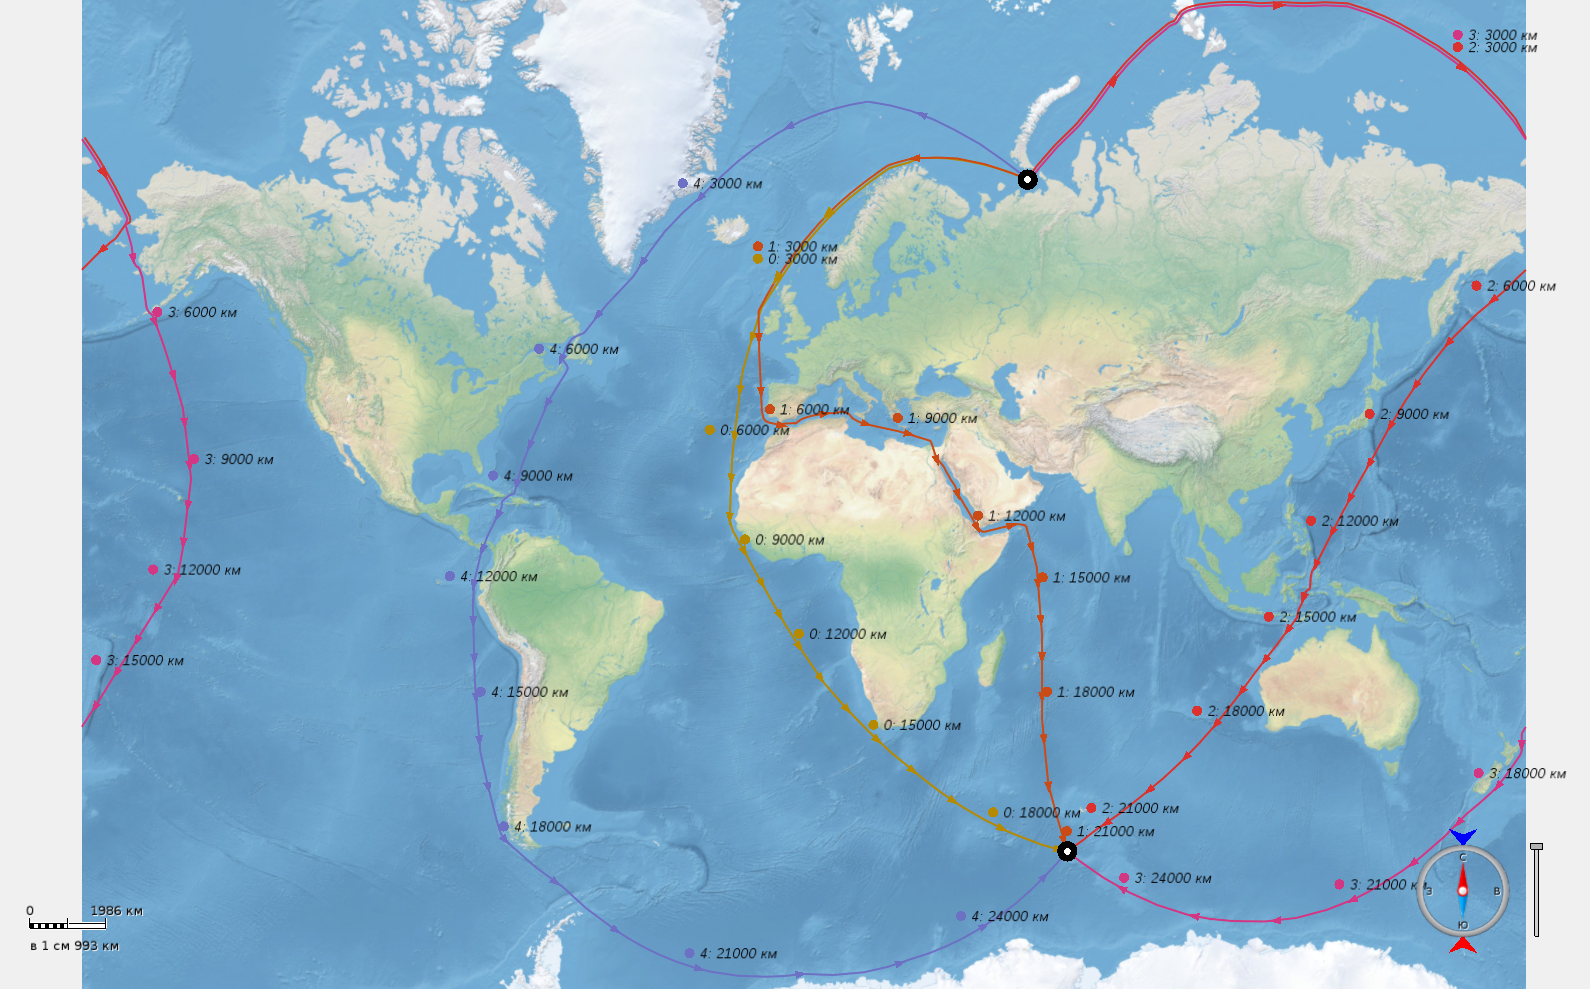
\includegraphics[width=.8\textwidth]{comparison-with-existing-good}
            \caption{Желаемый результат}
        \end{figure}
    }
\end{frame}
\note {
Известны различные алгоритмы поиска нескольких путей в графе. Однако все они не годятся для данной задачи.
Разрабатывались для других целей: например, поиск маршрутов по дорогам, поиск маршрутов на общественном транспорте, когда есть несколько способов добраться из точки А в точку Б. 
Не учитывают расположение: эти алгоритмы в большинстве своём оперируют абстрактными графами, не привязанными к конкретным координатам в мире.
Похожие маршруты: как следствие, попытка применить эти алгоритмы к данной задаче приводит к похожим маршрутам (хоть и почти не имеющим общих точек).
}

\begin{frame}{Предобработка данных}
    \begin{itemize}[<+->]
        \item Карта → полигон
        \item Смещение полигона внутрь
        \item Граф по сетке на плоскости + граф локальной видимости
        \item Ограничение длины ребра
        \item Дополнительные рёбра
    \end{itemize}
\end{frame}
\note {
1. Склеивание, упрощение. Полигон — множество контуров (в том числе дырок).
2. Корабли не плавают слишком близко к суше. Используется straight skeleton.
3. Чтобы находить кратчайший путь, нужен граф видимости. Но в нём
слишком много рёбер, поэтому построим навигационный граф. Разложим
вершины по сетке, проведём рёбра до соседей (и их соседей). Также
добавим вершины полигона и проведём из них рёбра до ближайших видимых 
вершин. Веса рёбер — расстояния между точками на сфере.
4. Путь ищется на сфере, при этом проверка корректности рёбер
осуществляется на плоскости. Кратчайшая траектория на сфере отличается
от кратчайшей траектории на плоскости. Не будем допускать слишком
длинные рёбра, тогда расхождение будет пренебрежимо мало.
5. Во-первых, добавим рёбра из straight skeleton'а, получившиеся в
результате схлопывания. Во-вторых, нужна возможность добавления рёбер
в связи с неточностями исходной карты. В-третьих, рёбра через 180-ый меридиан.
}

\begin{frame}{Поиск одного маршрута}
    \begin{itemize}
        \item<1-> Добавление вершин в граф
        \item<2-> Алгоритм Дейкстры
        \item<3-> Сокращение маршрута
        \begin{itemize}
            \item<3-> Если подпуть A → B → C можно выгодно заменить на A → C, заменяем 
            \item<3-> Подразбиение маршрута
        \end{itemize}
        \item<4-> Сглаживание маршрута
    \end{itemize}
    \only<5-5> {
        \begin{columns}
            \column{.5\textwidth}
                \begin{figure}
                    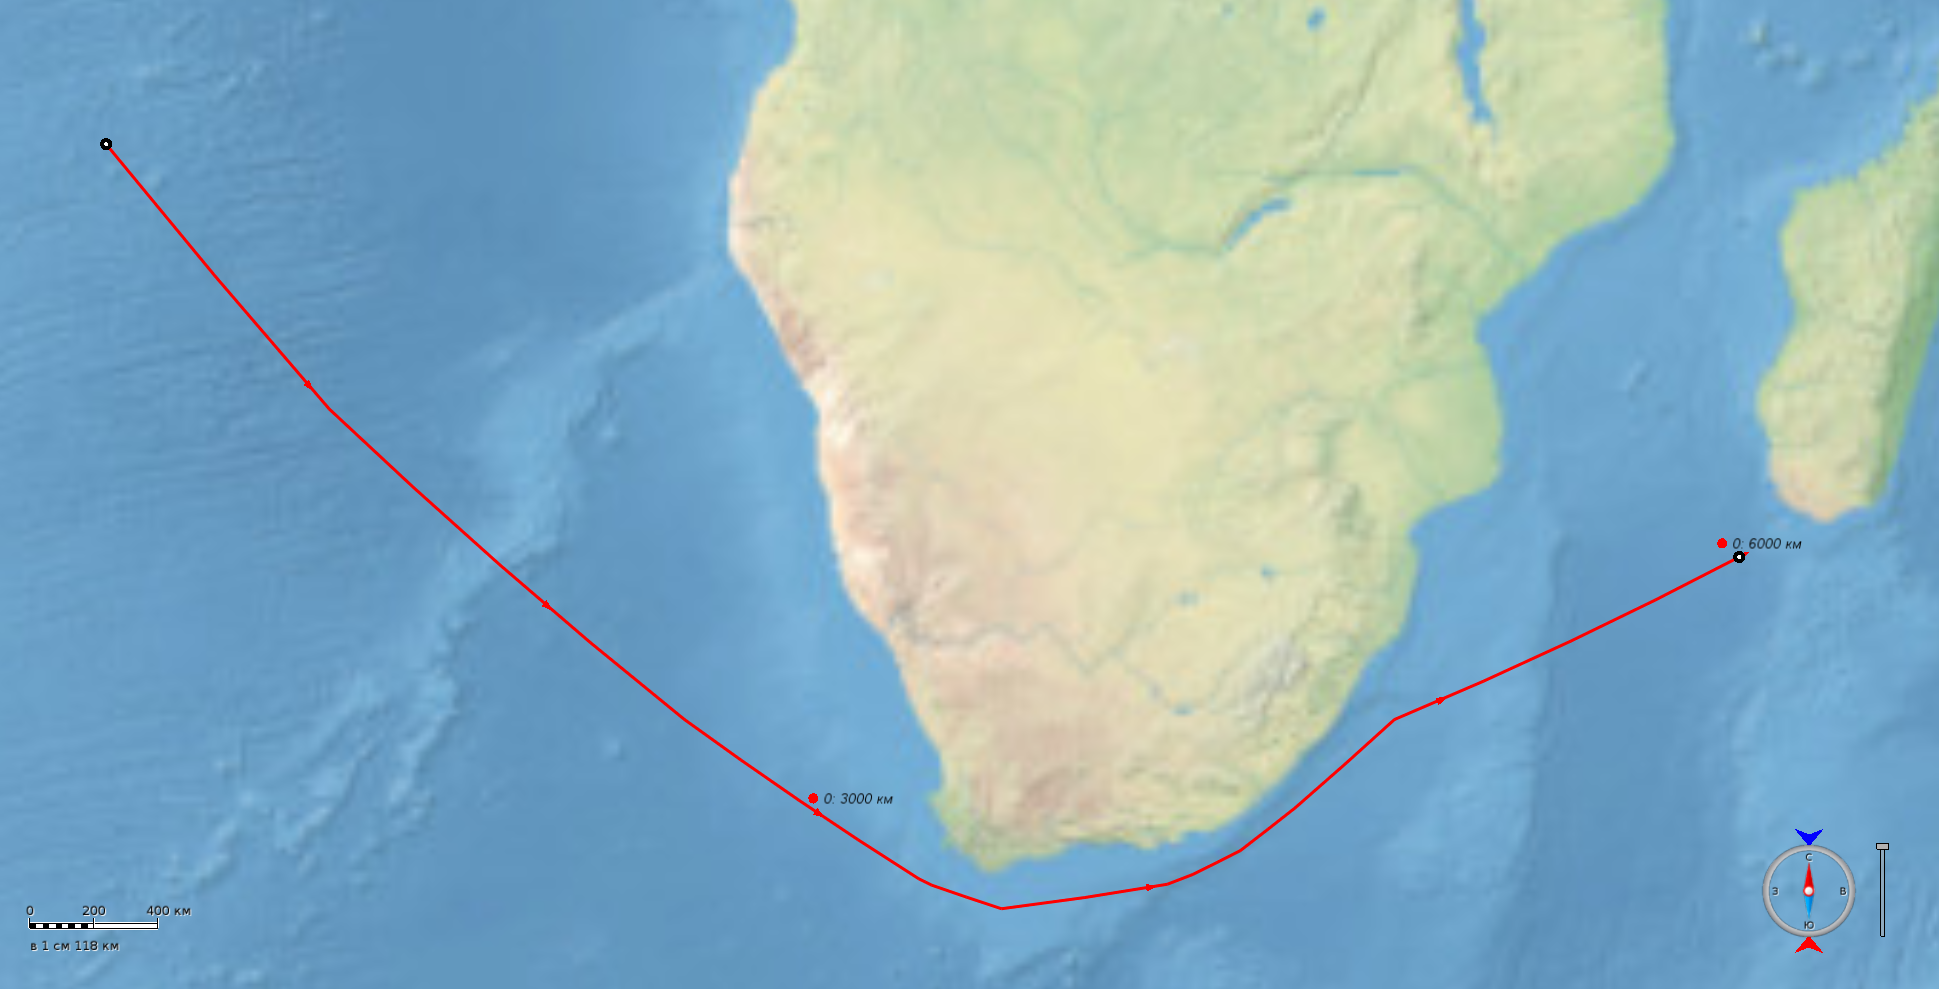
\includegraphics[width=\textwidth]{raw-path}
                \end{figure}
            \column{.5\textwidth}
                \begin{figure}
                    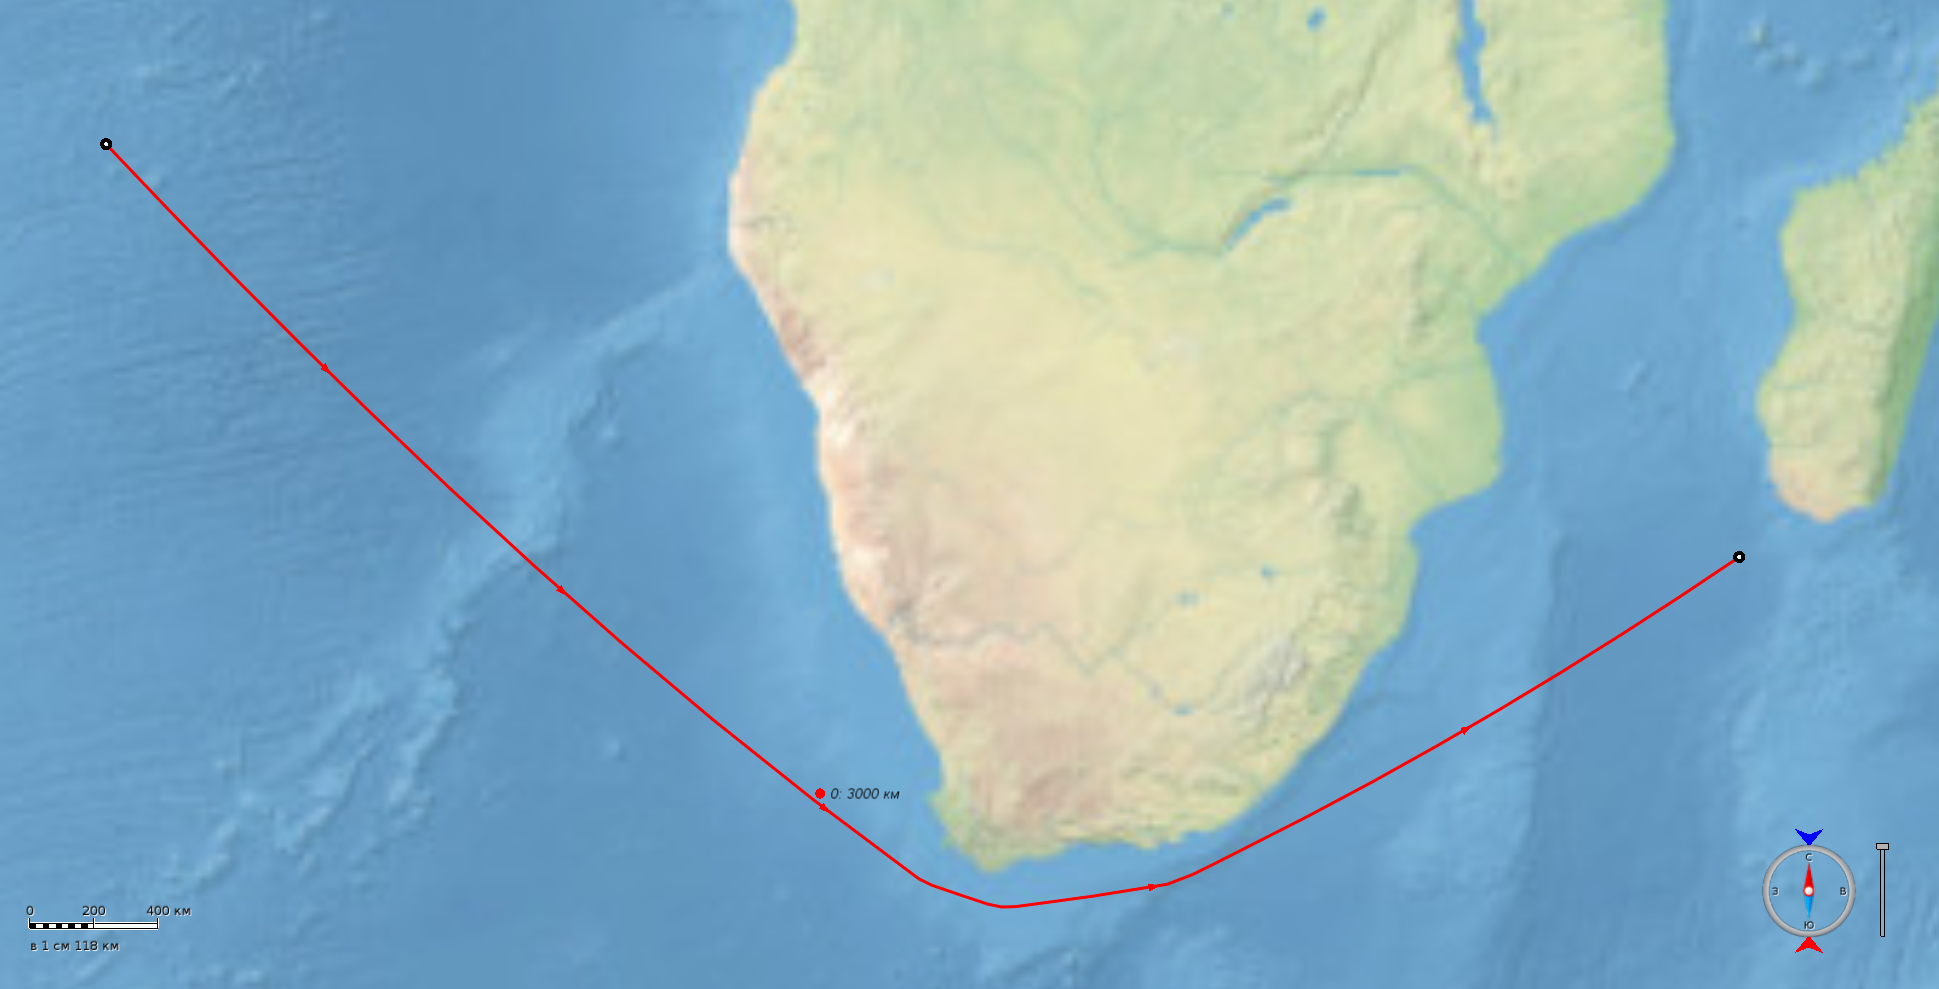
\includegraphics[width=\textwidth]{perfect-path}
                \end{figure}
        \end{columns}
    }
\end{frame}
\note {
Добавление вершин: проверяем, принадлежит ли воде. Добавляем вершину в граф. По сетке находим ближайшие вершины и добавляем к ним рёбра.
Сокращение маршрута: кратчайший путь в навигационном графе не обязан быть действительно кратчайшим путём. Обычно его можно сократить.
Сглаживание: избавление от очень острых углов, если это возможно (маршрут остаётся на воде). Из-за структуры графа могут возникать острые углы (резкие повороты). Реальные маршруты не такие.
}

\begin{frame}{Поиск нескольких маршрутов}
    \begin{itemize}
        \item<1-> Поиск одного маршрута
        \item<2-> Обновление весов:
        \begin{itemize}
            \item<2-> Потенциалы как функция кратчайших расстояний от фиктивной вершины 
            \item<2-> Обновление потенциалов
            \item<2-> Применение потенциалов
        \end{itemize}
        \item<3-> Проверка критерия остановки:
        \begin{itemize}
            \item<3-> Длина маршрута
            \item<3-> Метрики на маршрутах
        \end{itemize}
    \end{itemize}
\end{frame}
\note {
На этом слайде описана общая идея алгоритма.
Поиск одного маршрута: как сказано на прошлом слайде.
Обновление весов:
— из фиктивной вершины проводим рёбра нулевого веса во все вершины
пути. Запускаем алгоритм Дейкстры из фиктивной вершины, находим все
кратчайшие расстояния. Потенциал — эвристическая функция найденного
кратчайшего расстояния, определённая для каждой вершины (о ней позднее).
— обновление потенциалов (максимум/сумма/произведение/что-то ещё). Об этом тоже ещё скажу.
— обновление весов рёбер (модификация весов в соответствии с потенциалами).
Критерий остановки: определяем, хороший ли маршрут. Если хороший, то переходим к следующей итерации, иначе прекращаем.
— длина: если сильно длинее кратчайшего, то плохой.
— метрики: оцениваем похожесть на другие маршруты. Если есть похожий, то плохо.
}

\begin{frame}{Обновление весов}
    \only<1-1> {
        \begin{figure}
            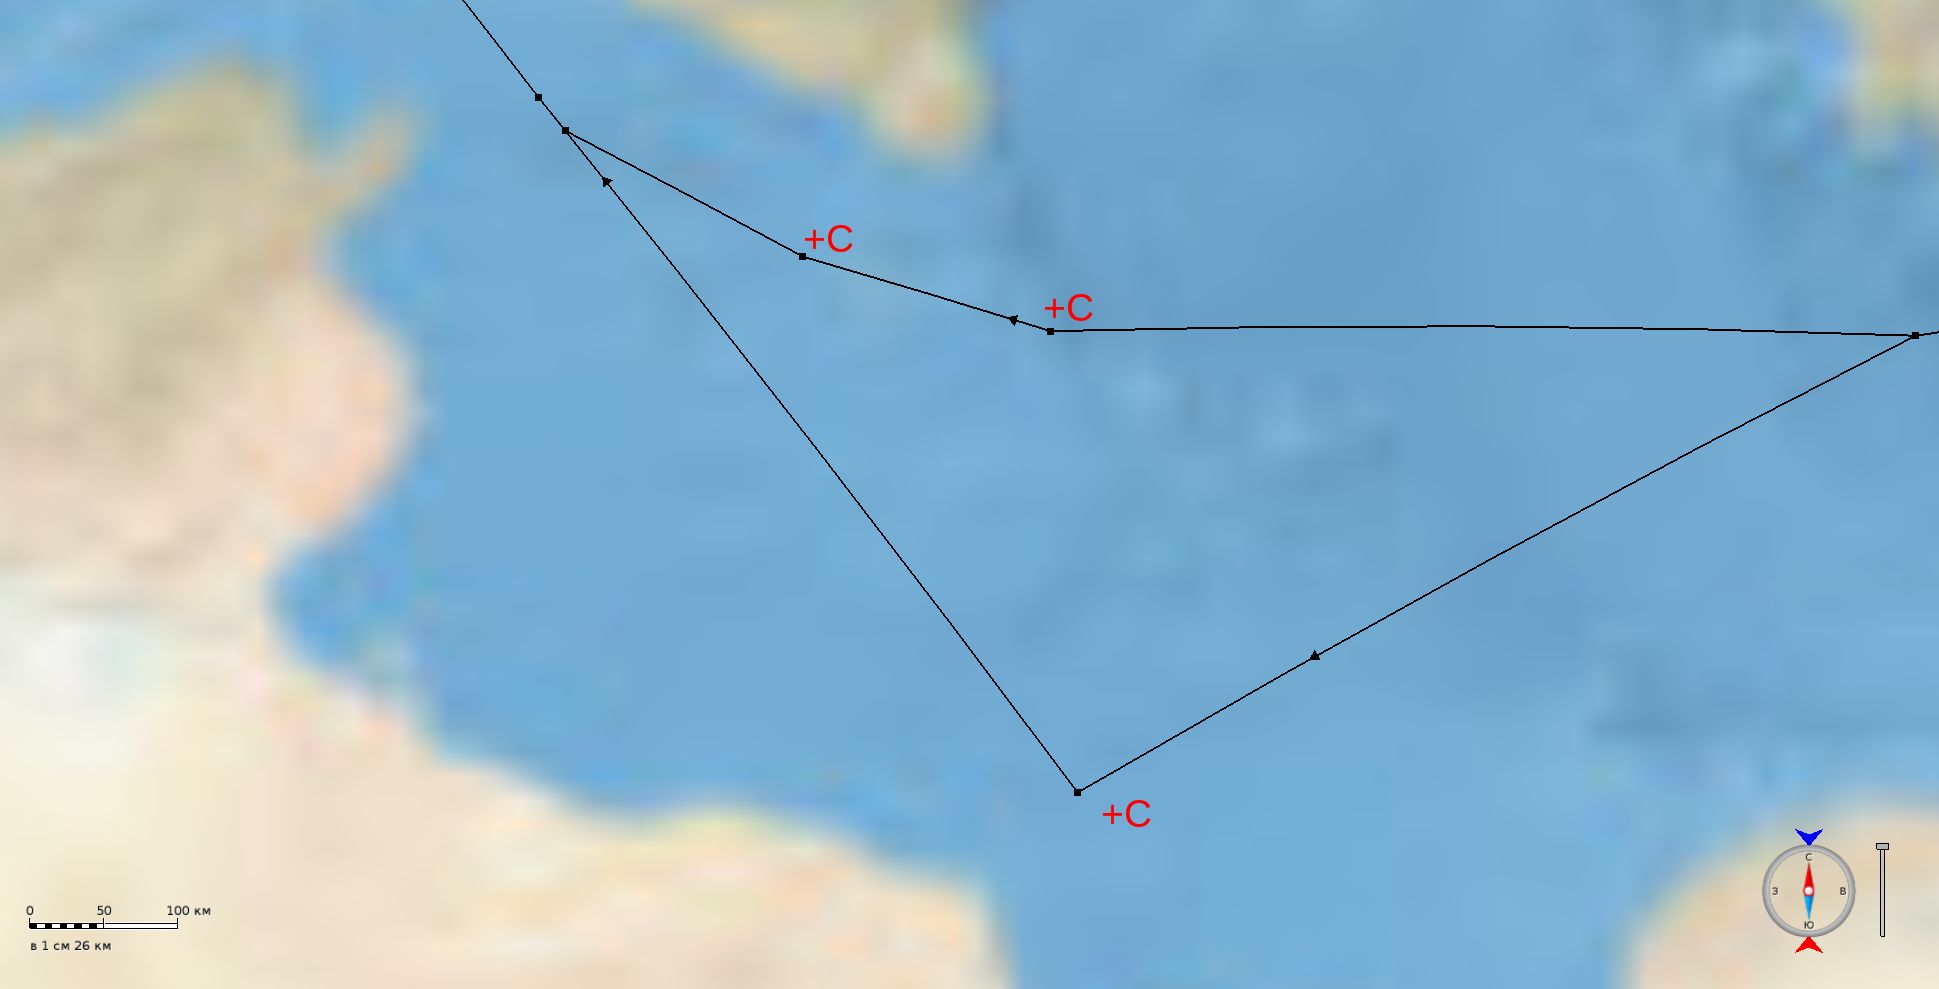
\includegraphics[width=\textwidth]{potentials-multipliers}
            \caption{Потенциалы должны быть множителями, а не слагаемыми}
        \end{figure}
    }

    \only<2-2> {
        \begin{figure}
            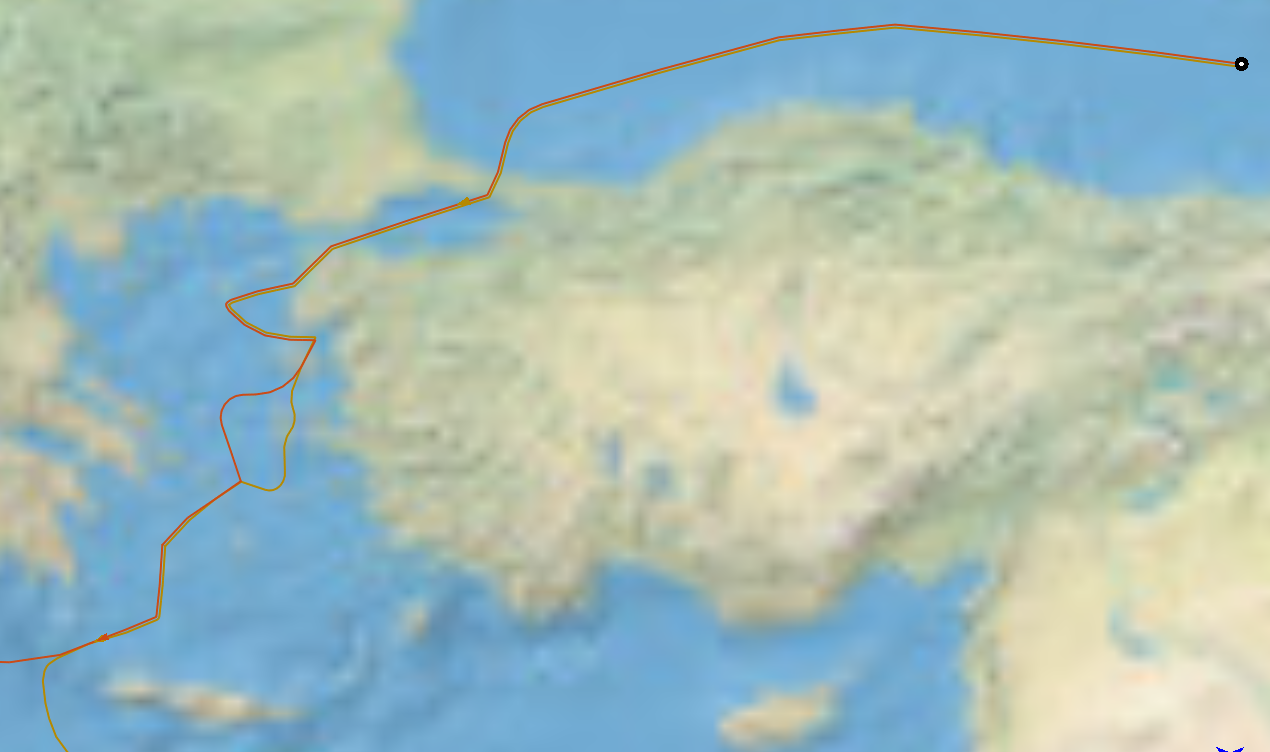
\includegraphics[width=\textwidth]{weights-on-path}
            \caption{На маршруте потенциалы меньше, чем поблизости}
        \end{figure}
    }
\end{frame}
\note {
На первой картинке видно, что если прибавлять потенциалы, то предпочтение будет отдано более длинному пути, состоящему из двух вершин, а не пути из трёх.
На второй картинке видно, что если не уменьшать потенциалы на маршруте, то результат будет неестественным.
TODO: показать, при обновлении потенциалов лучше брать максимум.
}

\begin{frame}{Метрики}
    \only<1-1> {
        \begin{equation*}
%        \begin{split}
            \rho_1 (P, Q) = \max(\max_{u \in P} \min_{v \in Q} \rho_g(u,
            v), \max_{u \in Q} \min_{v \in P} \rho_g(u, v))
%        \end{split}
        \end{equation*}
        \begin{figure}
            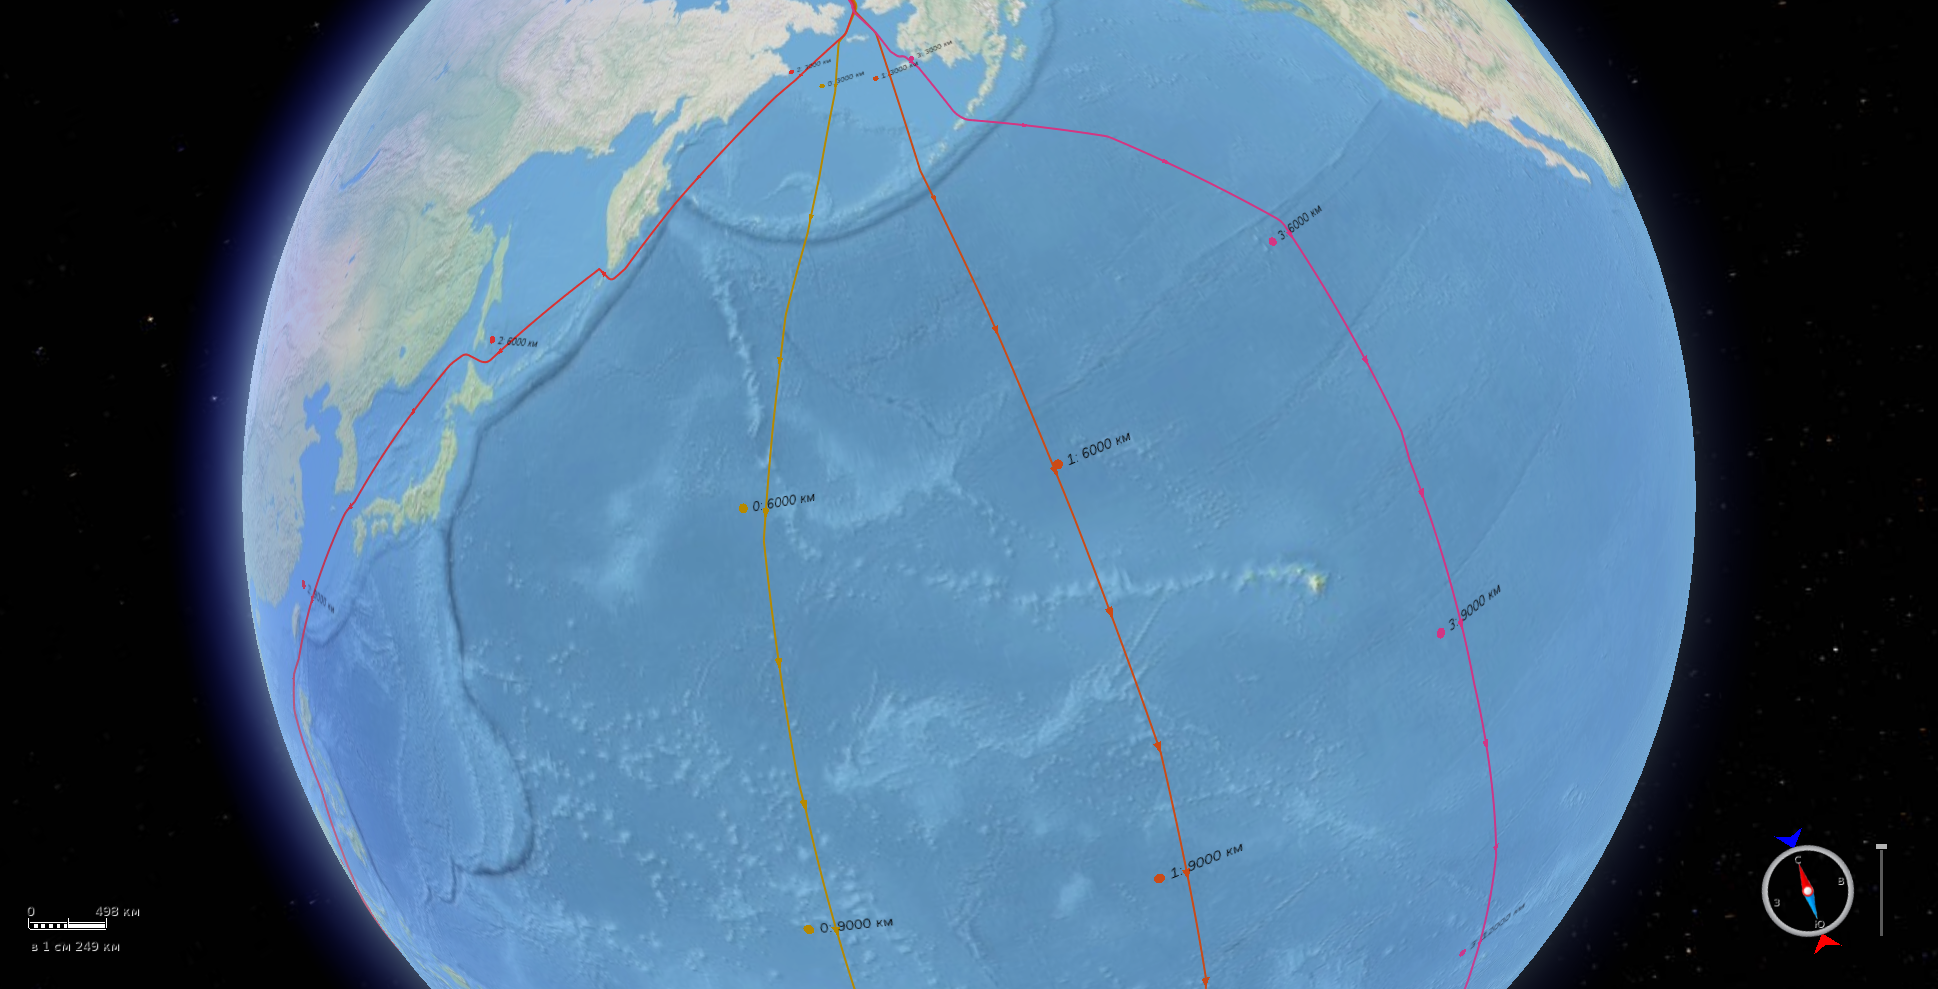
\includegraphics[width=\textwidth]{hg-definitely-similar}
        \end{figure}
    }
    \only<2-2> {
        \begin{equation*}
%        \begin{split}
            \rho_2 (P, Q) = \max(\max_{u \in P} \frac{\min\limits_{v \in Q_u}
            \rho_g(u, v)}{\min\limits_{v \in Q_u} \rho_r(u, v)}, \max\limits_{u \in Q} \frac{\min\limits_{v \in P_u}
            \rho_g(u, v)}{\min\limits_{v \in P_u} \rho_r(u, v)})
%        \end{split}
        \end{equation*}
        \begin{equation*}
            Q_u = \{ v : \rho_r(u, v) > \varepsilon \}
        \end{equation*}
        \begin{figure}
            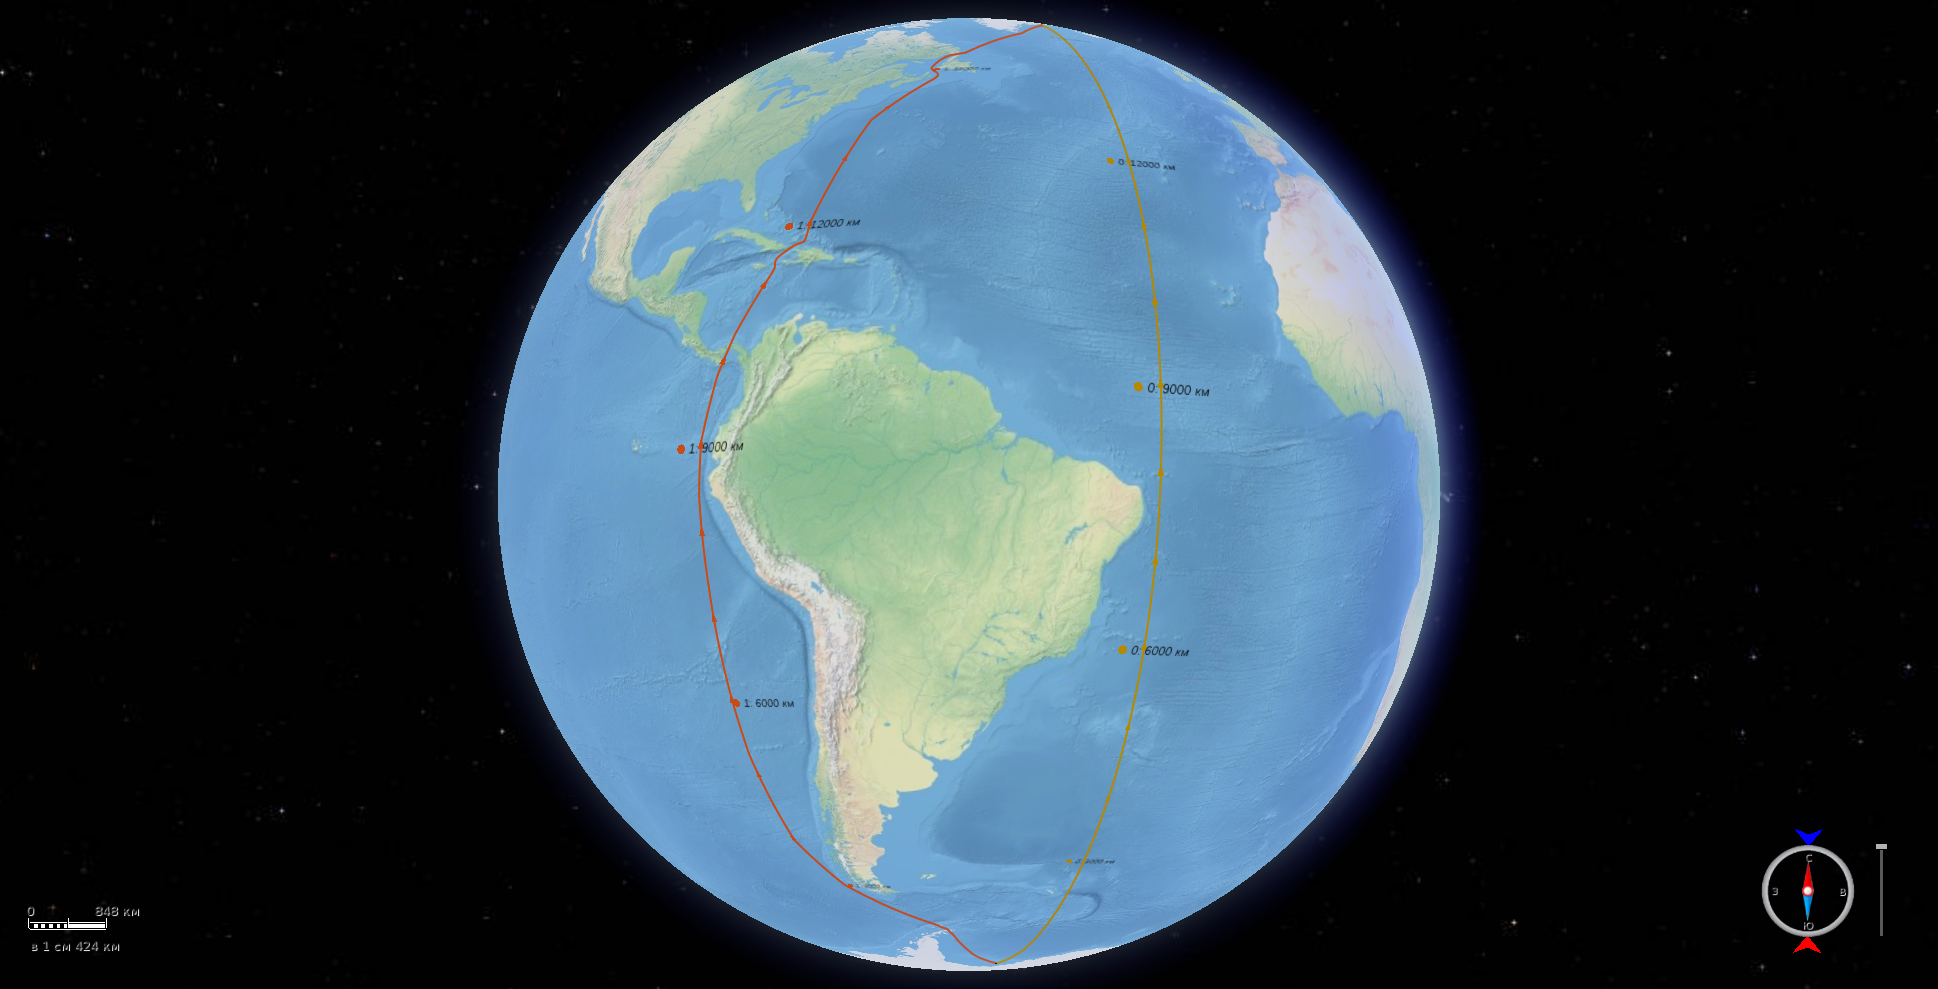
\includegraphics[width=.85\textwidth]{hg-maybe-similar}
        \end{figure}
    }
\end{frame}
\note {
Первая метрика: основная метрика для оценки похожести маршрутов. Если
значение очень большое (относительно длины маршрута), то маршруты
точно непохожи. Если значение очень маленькое, то маршруты точно
похожи. Иначе считаем, что значения этой метрики недостаточно.
Вторая метрика: дополнительная метрика. Нужна, чтобы различать
ситуации, когда мы обошли остров и когда между маршрутами просто так
получилось большое расстояние в смысле первой метрики.
}

\begin{frame}{Вычисление метрик}
    \begin{itemize}
        \item Фиктивная вершина
        \item Обход Дейкстры, пока не посещены вершины второго пути 
        \item Заканчиваем, если достигли необходимого значения
        \item Поиск ближайшей вершины (вторая метрика) — перебором
        \item На практике затраты как на первую, так и на вторую
          метрику небольшие
    \end{itemize}
\end{frame}

\begin{frame}{Результаты}
    \only<1-1> {
        \begin{itemize}
            \item Разработан и реализован алгоритм построения семейств оптимальных маршрутов 
            \item Проведено сравнение с существующими подходами 
            \item Поиск выполняется примерно за полсекунды 
            \item Используется в ПО «Кронштадт Технологии»
        \end{itemize}
    }
    \only<2-2> {
        \begin{figure}
            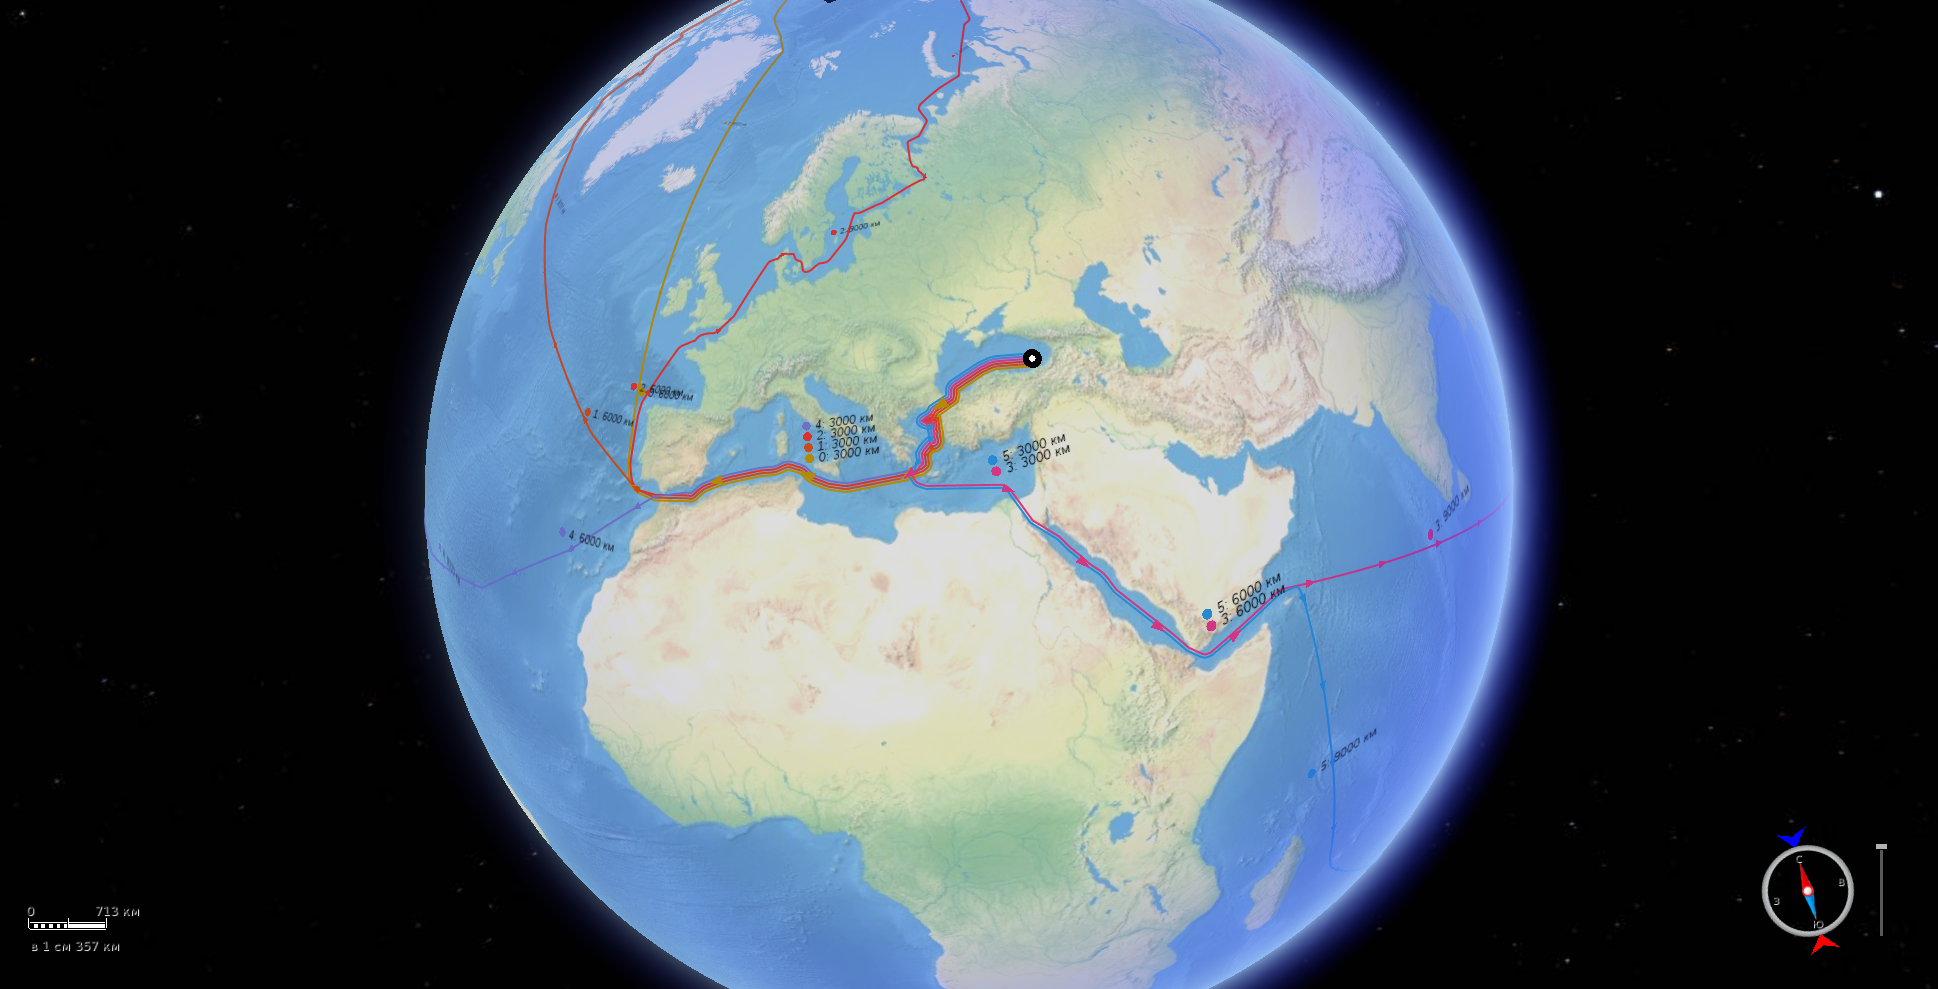
\includegraphics[width=\textwidth]{results}
        \end{figure}
    }
\end{frame}

\begin{frame}{Спасибо за внимание!}
    Вопросы?
\end{frame}
\note{До свидания!}

\end{document}

